


%-----------------------------------
%	SECTION 1
%-----------------------------------
\section{Interpreting high dimensional data}
\label{Intro-method} 
The evolution of genotyping and sequencing technologies led to the generation of high dimensional datasets. In Section \ref{Intro-ngs}, we have seen for example that arrays can interrogate thousands to millions of positions across the genome and that sequencing techniques can provide the entire genome sequence or the expression levels of thousands of genes. While the amount of information unveiled by these methods is colossal, it can also bring about several challenges and adapted computational methods are required to analyze and interpret the data. The issues resulting from high dimensionality are associated to what is called the curse of dimensionality, firstly introduced by Bellman in 1961 and stipulating that the number of samples needed to interpret high dimensional data analyses appropriately increases exponentially with the number of dimensions \cite{Altman2018}.  
In omics datasets, even though large cohorts have been implemented (see section \ref{Intro-ngs}), the number of variables (also known as features), $p$, to analyze can be largely superior to the number of samples, $n$, included in the study. This introduces the $n<<p$ problem, which leads to multiple issues.
Firstly, usual statistical models like regression models need to be adapted since they require $p<n$. There is also a substantial amount of noise in the generated data that can mask the true signal in the data, \textit{i.e.} not all the measured features are of interest \cite{Domingos2012, Ronan2016}.
In addition, when the number of dimensions increases, the data points can occupy a more voluminous space and a larger proportion of this space will be empty, we say that the data are sparse (See Figure \ref{fig:intro_highdim}) \cite{Altman2018}. High data sparsity influences basic properties to which we are used to in two or three dimensions like distances. In high dimensions, distances between points increase and all points seem at the same distance from each other \cite{Ronan2016,Altman2018}. Also, the higher the dimensions, the lower the correlations between the features will be. %For those reasons, it is thus statistically more difficult to identify groups of points with similar characteristics, and larger sample sizes are required. 
For those reasons, it is thus statistically more difficult to identify groups of points with similar characteristics compared with random events, as such larger sample sizes are required to distinguish meaningful relationships. Another issue resulting from high dimensionality is multi-collinearity. Since the number of features is high, the information they carry can be correlated and become redundant; some variables might be defined as a linear combination of others which makes the data interpretation more difficult \cite{Altman2018}. 
Finally, the nature of omics datasets complicates the visualization of the data.
In this section, we will discuss in a first instance different strategies to explore such complex datasets and secondly focus on methods that attempt to diminish the problem of the curse of dimensionality: the dimensionality reduction methods.

%Mention pvalue correction and the new discussion about pvalues and confidence intervals on twitter.
%Problem also of quality of the data, measurement errors

\begin{figure}[H]
    \centering
    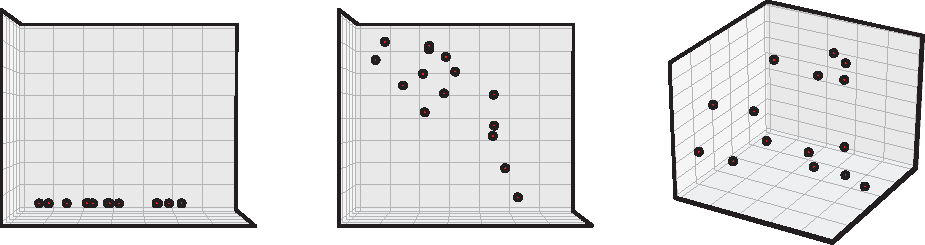
\includegraphics[width=0.8\textwidth]{Figures/Intro/high_dimentionality.pdf}
    \caption[Illustration of data sparsity]{\textbf{Illustration of data sparsity.} Figure from \cite{Ronan2016}. The figure represents how the data occupy the available space when going from a one-dimensional space to two and three-dimensional spaces (from left to right panels). }
    \label{fig:intro_highdim}
\end{figure}

\subsection{Supervised and unsupervised methods}

%Machine learning

Different approaches exist to analyze high dimensional data like omics data. In the case where specific biological hypotheses need to be tested, confirmatory data analyses based on inference models can be used. It can also happen that there are no predefined hypotheses and that the goal is to "let the data talk", in that case, \gls{EDA} will be more adapted \cite{Holmes}. A broad panel of statistical methods exists to assist both approaches. Among them, a large proportion can be grouped in the popular category of machine learning methods.  %In each case, different machine learning methods can be applied. 
The term \gls{ML} was used for the first time by Arthur Samuel around 1950 and defined a group of computer algorithms able to learn without being explicitly programmed to learn. Depending on the definition of learning, different classes of \gls{ML} methods have been established. In 1997, Tom Mitchell proposed a formal definition of algorithms learning saying that "A computer program is said to learn from experience E with respect to some class of tasks T and performance measure P if its performance at tasks in T, as measured by P, improves with experience E." \cite{Mitchell1997}. This definition matches a class of \gls{ML} methods, the supervised learning methods, used for classification and regression tasks. A common example is the identification of spam emails, where labelling emails in the spam or non-spam categories would be the task T, learning from a set of labelled emails would be the experience, and the proportion of correctly classified emails would be the performance measure P. However, \gls{ML} algorithms that simply learn from the input dataset without predefined ground truth (labelled data) also exist and are part of the unsupervised \gls{ML} methods. Those methods learn underlying structures in the data; hence algorithms like clustering or dimensionality reduction methods such as \gls{PCA}, which was developed even before \gls{ML}, are often included in the unsupervised learning category.
In the next paragraphs, both supervised and unsupervised learning are described (See Figure \ref{fig:intro_supervisedVSunsupervised}).  

\begin{figure}[H]
    \centering
    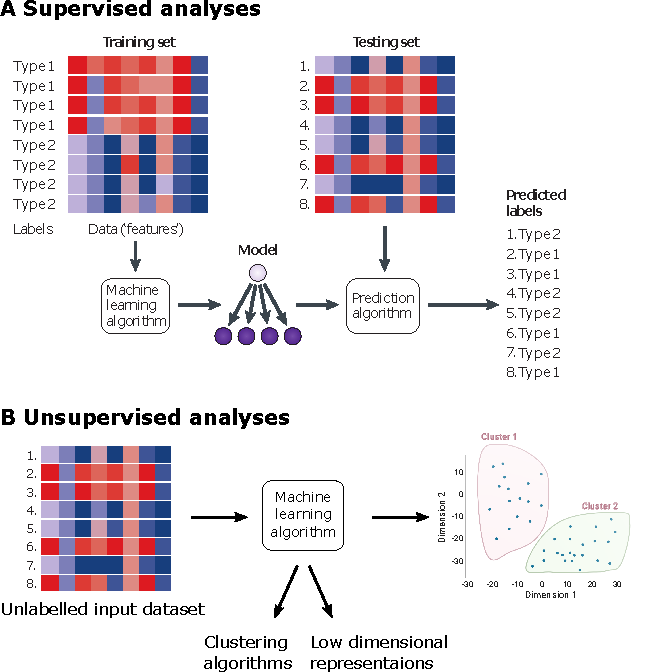
\includegraphics[width=1\textwidth]{Figures/Intro/supervised_vs_unsupervised.pdf}
    \caption[Machine learning methods: supervised vs non-supervised methods.]{\textbf{Machine learning methods: supervised vs non-supervised methods.} A) Supervised methods: a model is trained on several variables, features, to recognize predefined labels. The trained model is then applied to an unlabelled dataset for prediction purposes. B) Unsupervised methods: a model learns structures underlying a dataset that has not been labelled. Those methods are divided into two main categories: clustering methods to identify subgroups of samples and dimensionality reduction methods to explore the data in lower dimensions and highlight specific structures. Figure adapted from \cite{Libbrecht2015}. }
    \label{fig:intro_supervisedVSunsupervised}
\end{figure}

\textbf{Supervised analyses}
\newline 

The goal of supervised methods is to predict the value of an outcome based on a set of features given as inputs. Depending on the type of outcome, supervised analyses can be further divided into two main categories: classification or regression problems. In classification problems, the outcome is categorical, \textit{e.g.} a binary variable distinguishing a diseased or healthy status or a multi-classes variable like cancer subtypes. In regression problems, the objective is to predict a continuous variable. Note that some regression models, like logistic regressions, where the outcome variable is discrete, can be used though to perform classification.  
The main steps of supervised analyses consist in: i) defining the labels of each sample in the dataset, ii) train the model to classify the samples in the correct category, and iii) use the generated model on a dataset containing independent and unknown instances (Figure \ref{fig:intro_supervisedVSunsupervised}A). %Firstly, each element of the dataset has to be labelled, \textit{i.e.} each element belong to a pre-defined category. A machine learning model is then used to learn, from a set of variables, called features, how to classify each element in the correct category.
Several types of supervised methods exist and have to be chosen with regard to the nature of the data. The simplest supervised models are regression models. While the most common regression algorithms model linear relationships, other methods like \gls{SVM} or neural networks can adapt to non-linear data. Another parameter that determines the type of methods to use is the data type; some methods deal only with numerical features while others like decision trees are more flexible. Figure \ref{fig:intro_randomforest} describes a method based on decision trees, the random forest algorithm. 

\begin{figure}[H]
    \centering
    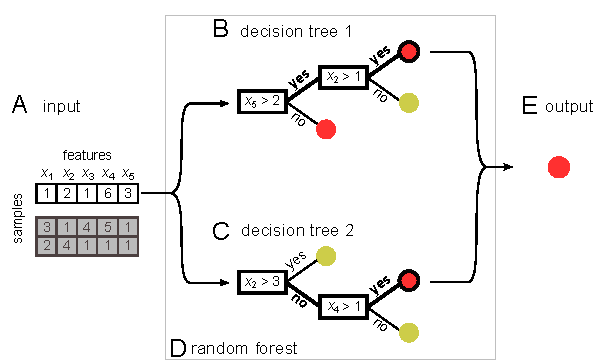
\includegraphics[width=0.8\textwidth]{Figures/Intro/random_forest.pdf}
    \caption[The random forest method]{\textbf{The random forest method.} Figure from \cite{Denisko2018}. A labelled dataset (A) is taken as input and processed by multiple decision trees (B and C) built using random selections of features and samples. The decision trees form a random forest (D). Each tree classifies the input samples and the votes given by the different trees are then combined to provide the final predictions. The label with the most votes being chosen (here red label). }
    \label{fig:intro_randomforest}
\end{figure}

%generalisation of the model
Regardless of the method used, the model and its results have to generalize to other datasets. In order to assess generalizability, the \gls{ML} algorithm has to be trained on a training dataset, and a testing dataset containing independent samples has to be used to validate the results. Two main errors underlying the generalization issue exist: bias and variance \cite{Domingos2012}. The first scenario occurs when the model is underfitting the data, \textit{i.e.} the model has a poor performance even on the training data for example because of a model that is not complex enough (See Figure \ref{fig:intro_biasVSvariance} left panel). When the model is underfitting the data, it is as well unable to generalize to other datasets. In the second case, when the number of features is too large or the number of samples small, the chances to encounter features that can perfectly discriminate two output categories or perfectly predict an outcome increase. The model, in that case, performs correctly on the training dataset but fails to generalize to other datasets and is qualified as high variance model. Such performance discrepancy indicates that the model overfits (See Figure \ref{fig:intro_biasVSvariance} right panel). Note that in high dimensional data, overfitting and data sparsity, resulting from the $n<<p$ problem mentioned at the beginning of this section, can be linked. Indeed, in such data, since the number of samples in the training dataset is fixed and limited, the entire input space is not covered. Thus the machine learning algorithm has not faced all possible configurations during the learning phase and the ability of the model to generalize can be diminished. 
\begin{figure}[H]
    \centering
    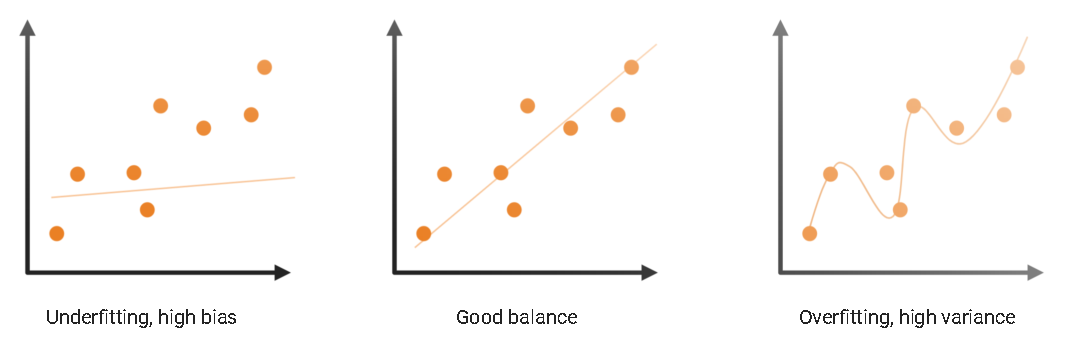
\includegraphics[width=0.8\textwidth]{Figures/Intro/overfitting.pdf}
    \caption[High bias and high variance models]{\textbf{High bias and high variance models.} Created with \href{https://biorender.com/}{BioRender.com}. }
    \label{fig:intro_biasVSvariance}
\end{figure}

One method that can be used to detect as well as overcome overfitting is cross-validation. The method consists in randomly splitting the dataset in $k$ folds and iteratively training the model on $k-1$ folds while reserving the remaining $k$th fold for testing (See Figure \ref{fig:intro_crossvalidation}). The overall performance of the model can be assessed by averaging the performances in the testing folds from each iteration. As a result, while none of the samples is used simultaneously in the training and testing group, the entire dataset is used for training as well as is used in the testing phase. Hence, cross-validation can also be beneficial in studies with low sample sizes. One extreme case of cross-validation is the leave-one-out analysis, where $k=1$. Each sample is set aside from the training set and predicted at each iteration. 
\begin{figure}[H]
    \centering
    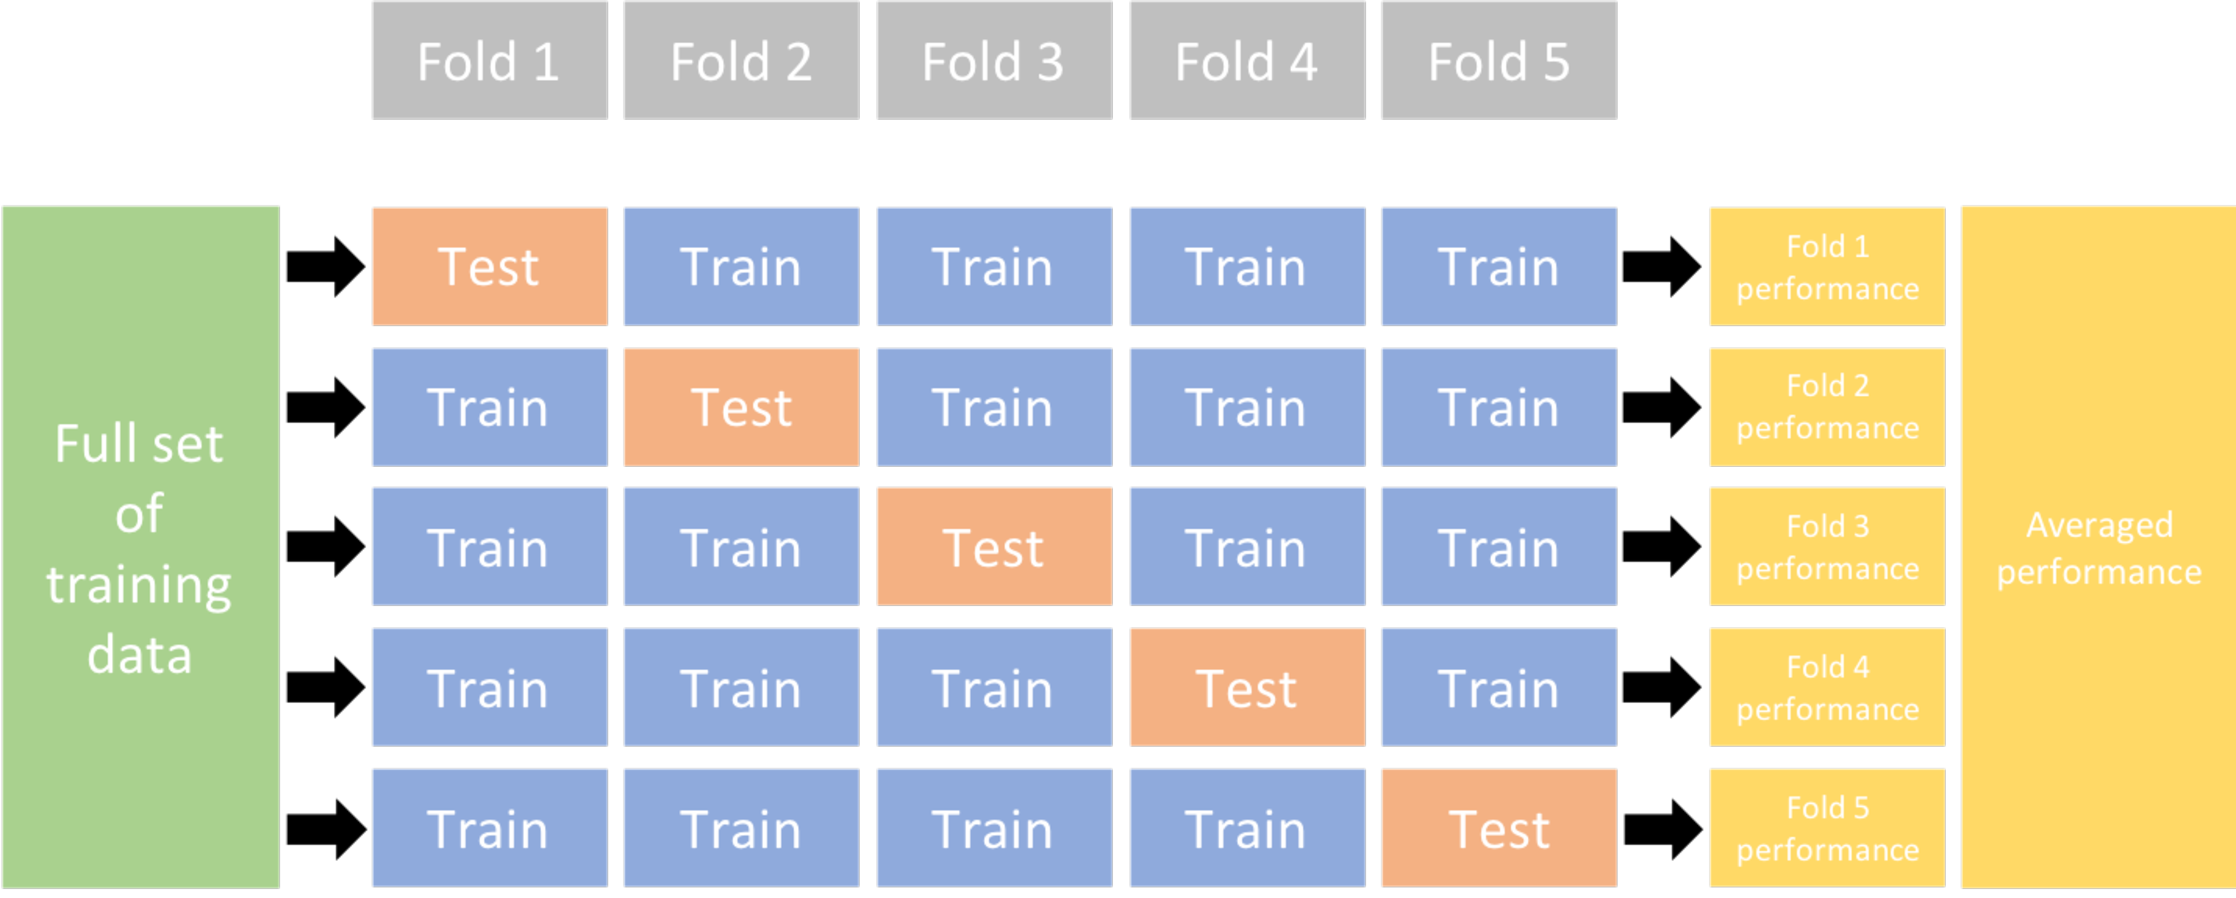
\includegraphics[width=0.9\textwidth]{Figures/Intro/cross_validation.pdf}
    \caption[$K$-fold cross-validation.]{\textbf{$K$-fold cross-validation.} Figure from \cite{BradleyBrandonGreenwell}. The figure illustrates 5-fold cross-validation. Five rounds are thus represented. In each of them, 4 folds are used to train the model and the model is tested on the remaining fold. The performances resulting from the test phase in each round are then averaged to estimate the overall performance of the model and its ability to generalize. }
    \label{fig:intro_crossvalidation}
\end{figure}

In addition, to find a compromise between bias and variance, parameter tuning and algorithm optimization might be required. Note that a third dataset, referred to as the validation dataset, can be introduced for the optimization step. In this setting, multiple models (\textit{e.g.} one algorithm with different sets of parameters or different algorithms) learn on the training set, and their performances are evaluated on the validation dataset. The model with the best performance can then be applied on the testing dataset.
\newline 

\textbf{Unsupervised analyses}
\newline 

Unsupervised algorithms are hypothesis-free methods and can be associated to exploratory analyses \cite{Oskolkov}. The goal of such methods is usually to identify and extract useful properties of the data \cite{Eraslan2019}. In contrast to the supervised methods, each element of the dataset is not labelled, no predefined groups are given to the algorithms. Thus, it is not possible to compare the algorithm output with a predefined truth and the data do not need to be split in training and testing datasets (Figure \ref{fig:intro_supervisedVSunsupervised}B). Since there is thus no feedback on the performance of the unsupervised model, often the validation of the results is required. 

As for the supervised analyses, there are several unsupervised algorithms. A commonly used category of unsupervised methods that can unveil structure in the data is the group of clustering algorithms (\textit{e.g.} $k$-means clustering, hierarchical clustering, density-based clustering). Those methods aim at grouping elements together based on common patterns observed in the set of features. In the field of cancer, clustering algorithms can be used, for example, to identify new subtypes of cancers based on molecular data. 
%Anomaly detection.
The second most commonly used unsupervised method is the group of dimensionality reduction methods. In the next paragraph, more details about such methods are provided.

%can generate hypotheses

\subsection{Dimensionality reduction methods}

The goal of \gls{DR} methods is to transform a high dimensional dataset into a low dimensional representation of the data while preserving as much as possible its initial structure. More specifically, if three clusters exist in the studied dataset, a lower dimensional representation of the same data should also reveal the initial three clusters. \gls{DR} methods are part of the feature extraction techniques which aim at finding latent structures in the data. Those methods allow to summarize and transform a large number of features in a smaller number of variables, which mitigates the curse of dimensionality and is valuable for data visualization. Note that these methods are different from feature selection methods, which make a selection of the most important features in the initial dataset \cite{Hastie2017}. Mainly two families of \gls{DR} methods exist: matrix factorization methods (\textit{e.g.} PCA, PLS, ICA, NMF) or neighbour graphs approaches (\textit{e.g.} t-SNE and UMAP). \newline


\textbf{Matrix factorization methods examples} \newline

Omics datasets, after pre-processing, often result in data matrices. For example, in the case of \gls{RNA-Seq}, after aligning the reads to a reference genome (See Figure \ref{fig:intro_ngs}), reads counting is performed and generates a matrix in which rows represent the genes (the features) and columns the read counts for each sample (the observations).  Matrix factorization consists in decomposing an initial matrix in two smaller matrices (Figure \ref{fig:intro_MF}). This decomposition leads to the generation of new variables, in smaller numbers. %In their review from 2018, Stein-O’Brien \textit{et al.} called the resulting matrices the amplitude and the pattern matrices \cite{Stein-OBrien2018}.
%In each matrix factorization method uses a different optimisation criterion to define the latent variables.

\begin{figure}[H]
    \centering
    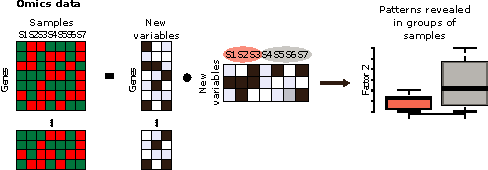
\includegraphics[width=0.9\textwidth]{Figures/Intro/MF_methods.pdf}
    \caption[Matrix factorization]{\textbf{Matrix factorization methods}. The input matrix is decomposed, under specific constraints, in two smaller matrices defined by new variables that can be used to reveal structures and patterns in the data.}
    \label{fig:intro_MF}
\end{figure}

A classical matrix factorization method is Principal Component Analysis (\gls{PCA}). The goal of \gls{PCA} is to project the data to a lower dimensional space while maximizing the variance in the data within this lower dimensional space. In \gls{PCA}, the new variables correspond to a linear combination of the initial features. The matrix factorization results in the loading and score matrices. In the first matrix, the columns correspond to the new variables, called principal components and the rows indicate the contribution of each feature to the latent variables. The principal components are orthogonal; they correspond to the directions of maximal variance and are ranked by the importance of variance explained, \textit{i.e.} the first principal component captures most of the variation in the dataset. The second matrix contains the coordinates of the samples in the projected space.
While \gls{PCA} maximizes the variance in the data, similar methods use other criteria. For example, \gls{ICA}, which is a method attempting at disentangling independent signals that are linearly mixed, maximizes the independence between the new variables. Other methods have in addition specific constraints \cite{Stein-Obrien2018}. \gls{NMF}, for example, enforces the decomposed matrices to be positive; this method has enabled the extraction of \textit{de novo} mutational signatures from whole genome sequencing data \cite{Alexandrov2013a}.
One limitation of those methods is that they are linear models. In the following paragraphs, two non-linear methods based on neighbour graphs are presented. \newline

\textbf{Neighbor graphs methods examples} \newline

The principle of \gls{DR} methods based on neighbor graphs models is to use neighbors distances and similarities to represent the structure of the data in high dimensions and then to embed this representation in a lower dimensional space. 

A method called \gls{t-SNE} \cite{VanDerMaaten2008} has been widely used in the past years to perform \gls{DR}. The \gls{t-SNE} method can be seen as a neighbor graph based algorithm \cite{McInnes2018} in a sense that similarity scores based on Euclidean distances between neighbors are computed to embed the high dimensional structure in a two-dimensional space. %The similarity between all the points is then calculated in the initial space and in the low dimensional space. 
Samples positions in the two-dimensional space are randomly initialized and are then moved iteratively so that the pair-wise samples similarities match the ones in the original space.  %Therefore, samples that are close to each others in the original space attracts each others.
\gls{t-SNE} has limitations though. Firstly, the method can be computationally intensive when applied to huge datasets. Also, the interpretation of the \gls{t-SNE} representation must be performed with caution. Indeed, the method retains local structures but has limited ability to maintain global structure \cite{McInnes2018}.  

Recently, a novel method called \gls{UMAP} \cite{McInnes2018} was developed and is more and more replacing the \gls{t-SNE} method. \gls{UMAP} is based on topological theory. The algorithm builds what is called a simplicial complex which is a representation of the data as a weighted graph (See Figure \ref{fig:intro_UMAP_topo}), the weights corresponding to the likelihood that there is a connection between two points \cite{McInnes_doc,AndyCoenen}.  
\begin{figure}[H]
    \centering
    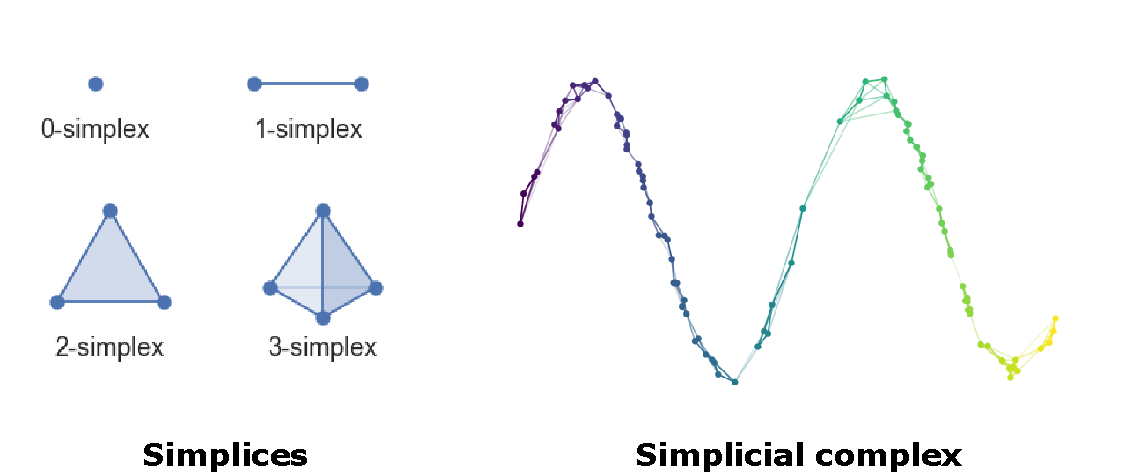
\includegraphics[width=0.9\textwidth]{Figures/Intro/simplicial_complex.pdf}
    \caption[UMAP topological representation]{\textbf{\gls{UMAP} topological representation}. A) The building blocks of a simplicial complex, the simplices. B) An example of a simplicial complex. Figures from \cite{McInnes_doc}.}
    \label{fig:intro_UMAP_topo}
\end{figure}
As mentioned at the beginning of Section \ref{Intro-method}, in high dimensional spaces data sparsity increases. To connect all the points in the simplicial complex, \gls{UMAP} varies the radius in which the search of neighbors is performed by fixing the number of neighbors to consider around each point \cite{McInnes_doc,AndyCoenen}. This number of neighbors influences how the data structure is preserved, low and high values favoring local and global structures, respectively. Once the graphical representation of the high dimensional data is constructed, a low dimensional representation of the data is optimized so that it is as close as possible to the high dimensional representation. % cross entropy
One of the advantages of \gls{UMAP} over \gls{t-SNE} is that the method better maintains the global structure of the data. Also, \gls{UMAP} is computationally more efficient \cite{McInnes2018}. Note that \gls{UMAP} can be applied on a lower dimensional dataset resulting, for example, from a \gls{DR} method like \gls{PCA}. 

% To connect each point to its closest neighbors, a radius is defined around each point and the points overlapping this radius are connected to the initial point. (using euclidean distance by default). 

%t-Distributed Stochastic Neighbor Embedding (\gls{t-SNE}), random initialization.  Computation of the similarity scores in the high and in the low representations. One of the problem of \gls{t-SNE} is that it does not scale to very large datasets.Also, the global structure of the data is not preserved, so inter-cluster differences can not be interpreted. Performing clustering on the resulting representation would not make sense. 

%To summarize, overcome overfitting issues and Dimensionality reduction methods help for the visualisation of such datasets \cite{DeAnda-Jauregui2020}. 
%Tmap: https://link.springer.com/article/10.1186/s13321-020-0416-x?shared-article-renderer

\subsection{Multi-omics data integration} 

The methods previously described consider as input a single dataset. \gls{DR} methods processing multiple matrices also exist and can be used to integrate multi-omics datasets. Such integration raises, though, multiple challenges. Firstly, the data to integrate are heterogeneous. The nature of the collected data is different, hence their statistical properties can vary. Also, it can happen that all the omics datasets are not available for each sample included in the analysis for technical reasons or due to quality issues. Hence, distinct patterns of missing data can occur in each omic dataset. Besides, integrating multiple datasets amplifies the curse of dimensionality issues already encountered in each dataset individually.

In 2018, a method called \gls{MOFA} was developed to integrate multi-omics data while considering the previously mentioned challenges \cite{Argelaguet2018}. \gls{MOFA} is an unsupervised analysis based on matrix factorization (See Section \ref{Intro-method}), and can be seen as an extension of \gls{PCA} to multi-omics data, called modalities or also views. It is a factor analysis method which reduces the dimensions of the data to a smaller number of unobserved factors, called the latent factors. These factors differ from the \gls{PCA} components. The latter are linear combinations of the initial features, while in factor analyses the initial features are expressed as linear combinations of the latent factors, plus a residual noise term. To enable multi-omics data (modalities) integration, \gls{MOFA} supports different noise models depending on the nature of the data (continuous, counts or binary data). Based on this model, \gls{MOFA} identifies different sources of variations across multiple omics data. \gls{MOFA} presents though several limitations. The model does not capture non-linear relationships and assume features independence \cite{Argelaguet2018}. %Also, the method does not account for additional information on the samples structure (groups of samples, batches, samples conditions) \cite{Argelaguet2018,Argelaguet2020}. 
Also, additional features accounting for samples structure, such as groups of samples, batches or samples conditions, were not available in the initial version of \gls{MOFA} but have been recently introduced in a second version, \gls{MOFA}+ \cite{Argelaguet2020}. In this framework, the \gls{MOFA} dimensionality reduction is performed with regards to additional samples information (\textit{e.g.} batch or cluster information) to identify sources of variations shared between groups or exclusive to one of them.
%In this framework, the method can, on top of integrating multiple omics data, also consider multiple samples groups \cite{Argelaguet2020}.

%The latter limitation can be overcome by other integrative methods. 
Other integrative methods can take into consideration samples structure. For example, the \gls{PLS} method, which is a matrix factorization method, attempts to relate two matrices: a response matrix and a matrix gathering explanatory variables. The advantage of this method is that it ensures that the new variables resulting from the dimensionality reduction explain the response data.
In that sense, the \gls{PLS} method can be considered as a supervised \gls{DR} framework. While \gls{PCA} maximizes the variance of the components, \gls{PLS} maximizes the covariance between the latent components of the response and explanatory datasets \cite{Kim,Hastie2017}. 
%The partial least squares (\gls{PLS}) method. 
When the response data is a categorical variable, a variant of \gls{PLS} called \gls{PLS-DA} can be used to perform classification tasks, \textit{e.g.} samples groups prediction. 
In 2017, Lê Cao team published the mixOmics framework implementing multivariate analyses tools, including the \gls{PLS} methods previously described \cite{Rohart2017}. The mixOmics tools also include the \gls{DIABLO} method, which is a multivariate dimension reduction method that can be used for supervised multi-omics data integration \cite{Singh2019}. \gls{DIABLO} maximizes the correlation between the features of the different omics datasets, one of this dataset corresponding to the labelled samples. Hence, the method extracts what the authors call multi-omics signatures that are discriminant and can be used for prediction in a supervised framework.  %However the method require parameter tuning lack from sparsity, see arguments from \cite{Argelaguet2018}


